\section{Jet Corrections in High Pileup Conditions}\hfill

As $\left<\mu\right>$ increases from 60 to 200 for the HL-LHC upgrade, the pileup contamination of hard scatter jets will begin to dominate. As PU contamination degrades the quality of HS jets, the task shifts from a binary classification at low pileup conditions to a continuous regression at high pileup conditions. Instead of the traditional binary labels as HS or PU, we introduce a continuous labels for Energy and Mass Fraction, Efrac and Mfrac, which represents the fraction of the jets energy and mass originating from pileup.

To construct these continuous labels, we sum over the Lorentz Four-Vector of the tracks, $\vec{T_i} = (E,p_x,p_y,p_z)_i = (E,\vec{p})_i = (T_0, T_1, T_2, T_3)_i$, which are truth-associated to each jet, $\vec{J}$:

\begin{equation}
    \vec{J}_{HS} = \sum_{i \in \text{HS}} \vec{T}_i \phantom{............} \vec{J}_{PU} = \sum_{i \in \text{PU}} \vec{T}_i \\
    %\vec{J}_{Total} = \vec{J}_{HS} + \vec{J}_{PU} 
\end{equation}

Now that we have the four vector HS and PU contributions of each jet, we can directly evaluate the Energy and Mass fractions on a per jet basis. The total Lorentz Four-Vector is simply the sum of the HS and PU contributions, $\vec{J}_{Total} = \vec{J}_{HS} + \vec{J}_{PU}$. Note that Energy is the first component of the jets Four-Vector, $J_0=E$, and mass is found using the relativistic energy relations in natural units, $m^2=E^2-|\vec{p}|^2$. These expressions can be used to derive the labels used for regression.

\begin{equation}   
    Efrac = \frac{E_{HS}}{E_{Total}} \phantom{............} Mfrac = \frac{m_{HS}}{m_{Total}}
\end{equation}

\begin{figure}[h]
\centering
\begin{subfigure}{.35\textwidth}
  \centering
  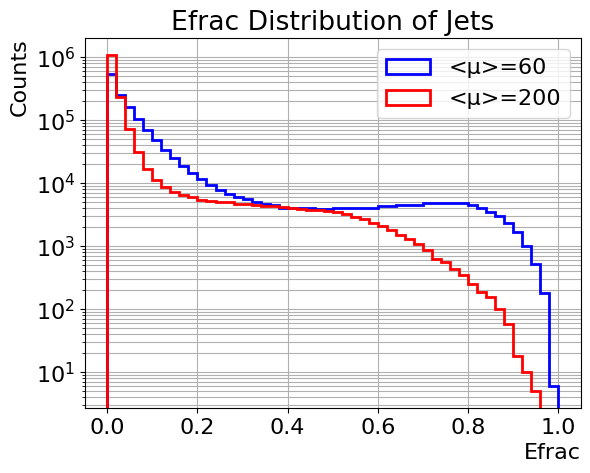
\includegraphics[width=1\linewidth]{Efrac}
  \caption{}
  \label{fig:sub1}
\end{subfigure}%
\begin{subfigure}{.35\textwidth}
  \centering
  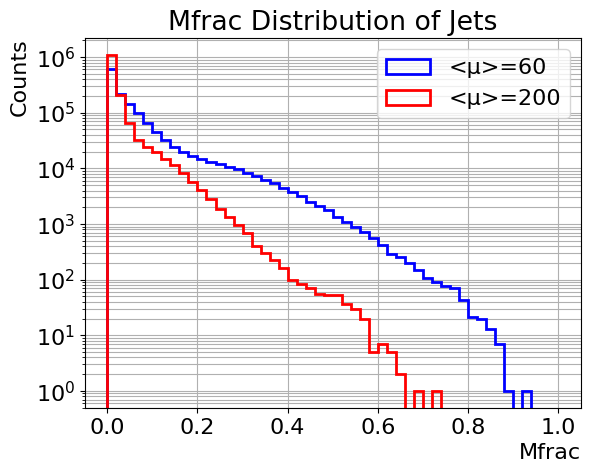
\includegraphics[width=1\linewidth]{Mfrac}
  \caption{}
  \label{fig:sub2}
\end{subfigure}
\caption{The truth energy and mass fractions used for the continuous regression task at $\left< \mu \right> = 60$.}
\label{fig:test}
\end{figure}

These continuous labels allow for corrections to be applied directly to the jet mass and energy. Of course a proper calibration will need to be applied when evaluated on data.
